% paper.tex | CS 6260 - "Vendetta" Paper

% setup
\documentclass[10pt,twocolumn]{article}
\usepackage{abstract}
\usepackage{color}
\usepackage{enumerate}
\usepackage{fullpage}
\usepackage{graphicx}
\usepackage{hyperref}
\usepackage{microtype}
\nonstopmode

% don't highlight links
\hypersetup{hidelinks}

% custom commands
\newcommand{\todo}[1]{\textcolor{red}{\textbf{TODO:} \emph{#1}}}
\newcommand{\term}[1]{\textit{#1}}
\newcommand{\bterm}[1]{\textbf{\textit{#1}}}
\newcommand{\code}[1]{\texttt{#1}}
\newcommand{\super}[1]{\textsuperscript{#1}}
\newcommand{\sub}[1]{\textsubscript{#1}}
\newcommand{\preta}{Pr\^{e}t \`{a}}
\newcommand{\pv}{\preta{} Voter}

% title
\title{Cryptographic assurance of secrecy and fairness in voting}
\date{}
\author{
  \begin{tabular}{c c c}
    Kelsey Francis &
    Curtis Free &
    Christopher Martin \\
    \small \tt{francis@gatech.edu} &
    \small \tt{curtis.free@gatech.edu} &
    \small \tt{chris.martin@gatech.edu}
  \end{tabular}
}

% document
\begin{document}
\thispagestyle{empty}

\twocolumn[
\maketitle
\begin{onecolabstract}

  Current election processes do not allow participants to verify the accuracy of vote counting.
  Applied cryptography research has yielded a number of candidate systems that replace or accompany
  existing voting procedures to provide fairness guarantees while maintaining ballot secrecy. We
	detail security properties necessary to make an election both ``fair'' and ``secret'' and analyze
	how three popular verifiable voting systems -- Scantegrity, \pv{}, and Helios --
	use cryptographic techniques to meet those goals.

\end{onecolabstract}
]

\section{Introduction}

Citizens' ability to trust the fairness of elections is vital to governments whose rule is subject
to the consent of the governed, but it is not uncommon for the veracity of election results to come
into question.  Current election processes do not allow participants to verify the accuracy of vote
counting.

Problems such as identity fraud and equality of ballot access are not amenable to cryptographic
solutions, but their propensity to be externally observable limits the potential for widespread
abuse.  Internal manipulation by the authority conducting the poll is a more insidious threat, and
it is here where we may fruitfully apply cryptography to ensure honesty. Research in this field has
yielded a number of candidate systems that replace or accompany existing voting procedures to provide
fairness guarantees while maintaining ballot secrecy.

In this survey, we study three of the most well-known solutions: the in-person voting systems
Scantegrity and \pv{} and the online voting system Helios.

First, we discuss the background of verifiable voting schemes and the security goals they
strive to satisfy. Second, we describe each of the three voting schemes in turn. We then
analyze their differing approaches to security and how well they achieve the desired goals. Finally,
we present some ideas that are not -- but perhaps should be -- considered by these schemes, and
we draw conclusions about the role of these schemes in elections today and in the future.

An election involves an information exchange between many independent \term{voters} and a single
\term{election authority}.
In a \term{verifiable} election, each voter may verify that her own vote was counted correctly
by the election authority.
A voter, or any other third party \term{auditor}, may also verify the accuracy of the final vote tallies
reported by the election authority. \cite{preta}
Voting is complicated by the requirement that all votes remain secret to avoid coercion.

\section{Verifiability}

\subsection{Verifiable recording}

When casting a ballot, a voter knows which candidate(s) she \emph{intended} to vote for -- but
once the ballot is cast, a system that supports verification of vote reporting allows the voter to
compare the recorded vote to what she intended to indicate on the ballot.

For example, at an in-person polling location -- ignoring ballot secrecy (see below) -- a voter
could be shown a screen giving the name of the candidate(s) she just voted for. If the display
does not match the voter's intention, then the voter can ``try again'' -- or call into question the
entire vote collection process.

\subsection{Verifiable collection}

After a ballot has been cast, and the voter has left the polling place, how can she be certain
that the ballot used in the final count is what she actually cast? (This could be a problem even
if the user has verified the \emph{recording} of the vote.)

It is possible -- as we shall see -- for a voting system to allow a voter to check that the ballot
she cast is exactly what was considered during vote counting.

\subsection{Verifiable counting}

Once votes have been collected, it is the responsibility of the state to tally votes for the various
candidates in a race and publish \emph{accurate} tallies. Generally, the electorate is reliant on
\emph{someone} to provide these tallies. But it is much less common for voters themselves to have
the opportunity to verify that the votes were tallied \emph{exactly} as they were cast.

These systems, however, allow publication of data sufficient to verify tallies. Relying on
cryptography to ensure secrecy, each system involves exposure of cryptographically-hidden vote
counts that can be used to ensure that -- given all votes cast -- the final tallies are correct.

\subsection{True cast ballots only}

While the notions of verifiability presented above allow one to ensure that votes were counted as
they were cast, another problem is to ensure that the body holding the election cannot fabricate
\emph{additional} uncast votes to raise the tallies as it sees fit.

\section{Ballot secrecy}

The intent of an election is to determine the true will of the voters.
If there is any possibility for a third party to discover the content of
an individual's ballot, then the voter's own will may be undermined by coercion.
Therefore a voting system must maintain secrecy of individuals' votes to avoid
the possibility that a voter may receive retribution or reward for casting a vote
in any particular way.

\cite{delaune} enumerates a hierarchy of ballot secrecy definitions.
In order of increasing strength, they are
\term{privacy}, \term{receipt-freeness}, and \term{coercion resistance}.

\subsection{Privacy}

Privacy addresses information that is revealed by the system itself.
A system is private if a voter who wants to keep her vote secret is able to do so.
In a verifiable voting system, the system includes the verification process.
So in addition to casting a vote in private, the voter must also be able to
audit her vote without revealing its content.

\cite{kremer} gives an \term{observational equivalence} definition of privacy:
An election system is private if an attacker, having access to the public
information published by the polling authority, ``cannot distinguish
the actual situation from one in which two voters have swapped their votes.''

% For all pairs of voters $v_1$, $v_2$ ...

\subsection{Receipt-freeness}

\subsection{Coercion resistance}

\subsection{Stuff that will be moved into one of the previous sections}

Countries such as the United States hold as a fundamental right that voting can be performed
in secret to reduce the possibility of voter coercion from any private entities.
In some developing states where corruption is prevalent, it may be desirable keep an
individual's vote hidden even from the election authority, again for the reason of
limiting coercibility. The latter goal is significantly more restrictive.

Ballot secrecy, often referred to as \term{receipt-freeness}, is perhaps the most complicated
security goal to address in a verifiable voting system.
Secrecy and verifiability are naturally at odds, and only through cryptography can we
reconcile these two requirements.

Amidst these other goals, it becomes difficult to prevent \term{coercion}: the ability of some party
to coerce a voter to vote for a particular candidate.

With conventional in-person voting, coercion is thwarted to some extent by the physical security
imposed at polling locations: a party cannot \emph{watch} a voter cast a ballot and so cannot rest
assured that the voter did as told.

Though ballot secrecy prevents such a party from determining that a voter has done as asked, it is a
different problem to ensure that even the voter herself cannot prove that her ballot was
cast a certain way. We show, in describing these systems, that the cryptographic techniques
used to provide ballot secrecy also ensure -- in the case of in-person elections -- that a voter
cannot prove her ballot was cast a certain way even with the data necessarily exposed to provide
verifiability.

\section{Scantegrity}

The Scantegrity system \cite{scantegrity_ii} -- we consider an updated version technically known as
Scantegrity II -- is designed to provide verifiability atop existing in-person voting systems that
rely on fill-in ballots processed via optical scan.

\subsection{Before voting}

Before an election is held, the election authority must construct four Tables that lie at the core
of the Scantegrity system: Tables P, Q, R, and S.

Some selection of officials conducting the election use a secret-sharing scheme to protect a
secret pseudorandom number generator key. Table P lists every ballot that will be produced for the
election and specifies exactly what code is used for each candidate per ballot. These codes are
generated using the pseudorandom generator and \emph{must} be kept secret.

Table Q has one row per ballot, as in Table P, but the codes presented on that ballot are included
in randomly-ordered cells so that a particular code cannot be mapped to a particular candidate.
Once ballots have been collected, only the cell actually marked on each ballot is revealed. (Note
that the column shuffle must be per-row, as otherwise one could determine whether two voters
cast a vote for the same candidate.)

Table S contains final vote tallies. Each column represents a particular candidate, and there will
be one ``checked'' cell in each column for each ballot cast for that candidate.

Table R comprises the heart of the Scantegrity Tables: it maps cast ballots in Table Q to tally marks
in Table S. Each row in Table R maps a single cell in Q to a single cell in S, and the order of
these mappings is pseudorandom (though the mappings must obey the data specified in Table P for vote
correctness).

After these tables have been generated, the election authority must \term{commit} to their contents
so that any change from this point forward is impossible or detectable.

It is at this point that the election authority audits a selection of the ballots; this is discussed
further in our analysis.

\todo{Include our own depiction of the tables in an image.}

\subsection{Voting}

A Scantegrity ballot consists of two portions: a special optical-scan ballot strip and a second
piece of paper that the voter will keep as a receipt. Each ballot is identified by a unique number,
which is printed on both portions. (While this number can be printed in plain sight, it can also be
encrypted on the optical-scan portion such that someone with physical access to a ballot box cannot
link a particular ballot to a voter with receipt in-hand.)

All candidates are listed on the optical-scan ballot, and the voter makes her choice by filling
in a ``bubble'' that reveals an alphanumeric confirmation code (as specified in the private Table
P), which the voter then records on the receipt portion. The ballot is sent through an optical
scanner, and the voter takes her receipt when leaving the polling location. It can later be
compared against published Table Q to ensure that the vote was recorded properly.

Additionally, during the voting process, a voter can ask a poll worker for an second ``audit''
ballot. This ballot is initially just like any other ballot: however, \emph{all} candidate codes are
revealed, and the ballot is marked as an audit ballot. An audit ballot is scanned, but the voter is
allowed to keep the ballot for later verification. This verification process is described and
discussed in our analysis.

\subsection{After voting}

When a ballot has been received, the following takes place:
\begin{enumerate}
	\item
		The candidate code is revealed in Table Q. (If this is an audit ballot -- see below -- then all
		are revealed, and we'll perform the following steps for each code.)
	\item
		A ``check'' is placed on the row in Table R that maps the revealed Q value to some value in S.
	\item
		The Table R mapping is followed into Table S, and a ``check'' is added to a cell in Table R,
		to be counted as a vote for that row's candidate.
\end{enumerate}

Tables Q and S and published in their entirety. However, one member of each Q-to-S cell mapping pair
is hidden prior to its publication (except for audit ballots, for which both sides of the mapping
are revealed). This data is required for third-party verification.

We further discuss this process in our analysis.


\section{\pv{}}

\pv\ aims to offer a familiar, in-person voting experience while providing cryptographic assurance of
a fair election.

\todo{Fill in.}

\section{Helios}

Helios \cite{helios} -- unlike Scantegrity and \pv{} -- is an \emph{online} voting
system; however, it, too, is designed with an emphasis on verifiability.

\subsection{Before voting}

At the heart of Helios is a single ElGamal key pair. The secret key is known only to the Helios
server, but the public key can be accessed in some way by all participants.

\subsection{Voting}

When a voter goes to cast a vote, her candidate selection is encrypted locally (i.e., on her
computer terminal, in the browser) using ElGamal. Prior to casting the ballot, the voter is
presented with a SHA-1 hash of her encrypted ballot. At this point, the voter may choose either
to submit the ballot or to ``audit'' it. In the former case, the ballot is cast and voting is
complete. But when a voter chooses to ``audit,'' she is presented with \emph{all} of the data
used to encrypt the vote. Namely, this includes the public key and the ``randomness'' that were used
by an implementation of ElGamal to encrypt the vote. The voter can then -- using a modified ElGamal
which allows randomness to be specified -- perform the encryption and SHA-1 hash herself
to verify that the hash that \emph{would} have been cast actually does represent the ballot she
intended to cast.

\subsection{After voting}

Once all ballots have been collected by the Helios server, they are shuffled by a cryptographic
``mixnet.'' \todo{We should discuss re-encryption details, which are covered in the Helios paper.
Maybe we cover the details in the \pv{} Voter discussion?}

\begin{figure}
	\center
	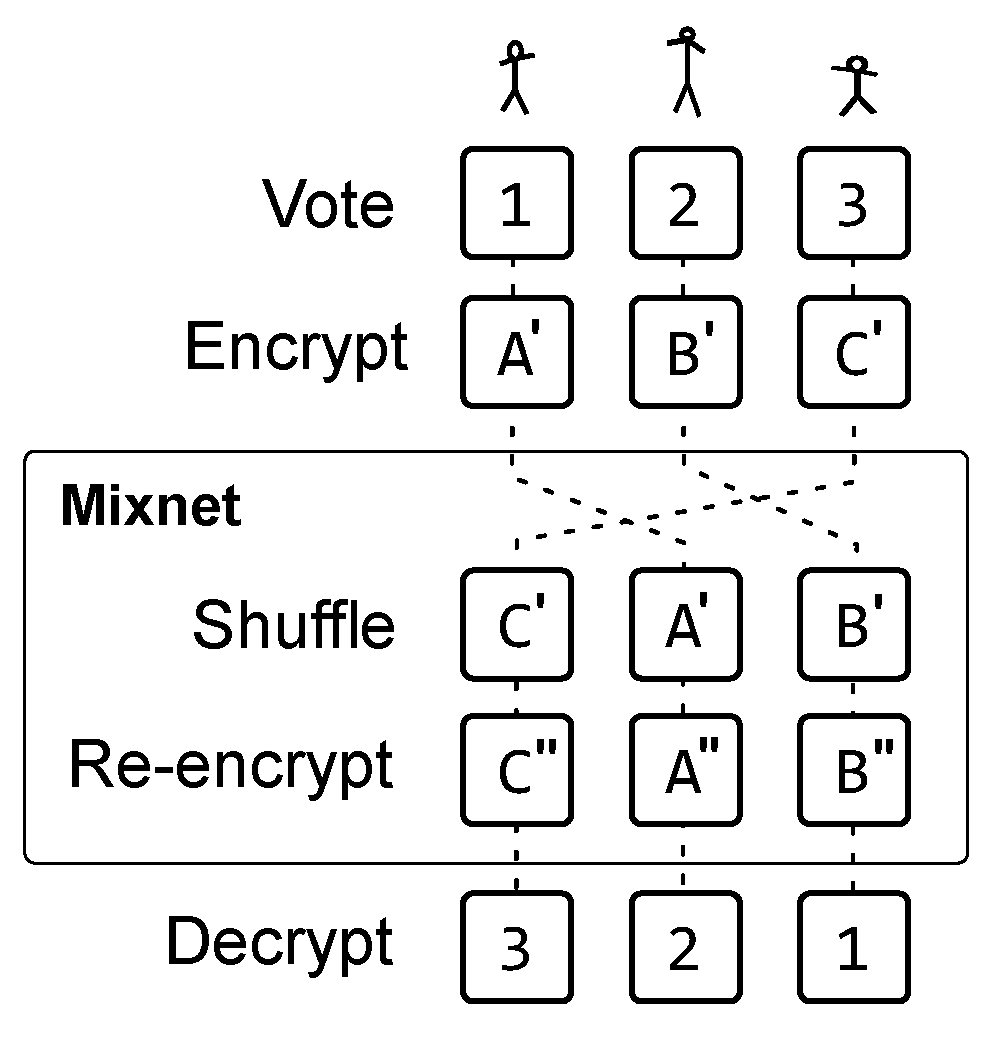
\includegraphics[width=0.8\columnwidth]{images/include/mixnet.pdf}
	\caption{A re-encryption \term{mixnet}}
	\label{fig:mixnet}
	\vspace{-25pt}
\end{figure}

The ``mixnet'' accomplishes two goals: it shuffles the votes \emph{and} re-encrypts them (with the
same key, but with different random inputs). A random permutation -- referred to as $\pi_{N}$ (where
$N$ is the total number of votes) -- is first used to perform the shuffle. Each ciphertext
$c_{i}$ is then ``re-encrypted'' to a new ciphertext $d_{i}$ that equivalent to the first \emph{had
the random input at encrypt time been different} by a particular amount $s_{i}$. See Figure
~\ref{fig:mixnet} for a visual depiction of this process.

The ``shuffling'' is important because it prevents an attacker from linking a decrypted ballot with
a particular encrypted ballot -- and thus a voter. Re-encryption means that an auditor examining a
proof of proper decryption cannot determine how a particular voter cast her ballot by hashing
all ciphertexts in the proof and matching those hashes to the publicly-posted encrypted vote hashes.

Finally, votes are decrypted and tallied. At this time, Helios also publishes the information
necessary for anyone who wishes to audit the election to verify that the mixnet's shuffling and
decryption were performed properly.

In order to provide a guarantee of proper shuffling, Helios actually shuffles the votes multiple
times, actually using only the final shuffle in tallying the results. The other shuffles are
referred to as ``shadow mixes'' and are made public. Those mixes are hashed to obtain a bit string
that is used, bit-for-bit, as a set of challenges, with one bit value indicating that Helios must
provide the permutation used for the shuffle and the $s_{i}$ values used for re-encryption, and the
other bit value indicating that it must provide a mapping from one shadow mix to another. This is
known as an ``Honest-Verifier Zero-Knowledge'' proof, for which the probability that the final
product is correct is equal to $1 - 2^{t}$, where $t$ is the number of shadow mixes produced.

Similarly, the Chaum-Peterson zero-knowledge proof technique is used to prove that decryption is
correct. \todo{How much detail should we provide?}

\section{Analysis}

We analyze these voting systems by considering each security goal in turn.

\subsection{Ballot secrecy}

Each of these systems provides ballot secrecy by performing a three-step process:
\begin{enumerate}
	\item
		Encrypt ballot prior to its being cast.
	\item
		``Mix'' the ballots in some way.
	\item
		Reveal decrypted ballots for tallying.
\end{enumerate}

\subsubsection{Encryption}

In both Scantegrity and Helios, the following information is revealed after the election:
\begin{itemize}
	\item
		\emph{Some} information about \emph{all} encrypted ballots, linked to voters.
	\item
		\emph{All} decrypted ballots, \emph{not} linked to voters.
\end{itemize}

In Scantegrity, ``public'' version of a ballot is really just an encryption of the voter's
selections: it is an independent, uniformly random code chosen beforehand and corresponding to a
particular candidate for that ballot. Table P defines an explicit, ``keyless'' encryption
function -- and each ballot holds just enough information from Table P to encrypt a single voter's
responses. (Alternatively, one can think of Table P as an encryption scheme definition wherein the
ballot number is the key. However, the table is a collection of \emph{all the keys}, and its
compromise would eliminate ballot secrecy for all ballots.)

In Helios, the ``public'' ballot is a hash of an encryption. Helios uses ElGamal to encrypt ballots,
which -- unlike Scantegrity's core \emph{random} Table P -- could be subject to attack, given that
ElGamal is a published encryption function. Similarly, Helios uses the standard SHA-1 hash algorithm
to hash encrypted ballots. Note that we are not making a precise quantification about Helios's
security: rather, we simply note that the difference between these two systems can be thought of as
a tradeoff between key size and privacy guarantees. Scantegrity essentially has an immensely large
key that -- because it is theoretically completely random -- ensures that ciphertext cannot be
decrypted. Helios, however, uses known algorithms with shorter keys that could potentially be
attacked. Compromise of keys in either system would destroy their privacy guarantees.

\subsubsection{Mixing}

Essentially, both Scantegrity and Helios use some mechanism to ``shuffle'' votes so that -- even
with votes decrypted for tallying -- encrypted ballots cannot be linked to their plaintext
counterparts.

In Scantegrity, the ballot ``mix'' is predetermined, as it is defined by the generation of Table R.
When that table is constructed, ballots are pseudorandomly ordered. With the exception of audit
ballots, the information revealed that is ultimately revealed allows half of the ballots to be
traced only from Table Q to Table R; and the other half can only be traced from Table R to Table S.
Should Table P be compromised, one could complete all mappings and violate secrecy entirely -- or
simply decrypt encrypted votes with no attention giving to Table R. Should the mapping on
\emph{either} size of Table R to votes in Table Q \emph{or} tallies in Table S be deterministic,
privacy would be compromised for half of all voters.

Where Table R lies between encryptions and decryptions in Scantegrity, Helios makes use of a
cryptographic \term{mixnet} -- performed with cast ballots in hand -- to prevent an attacker from
tracing a vote to its decryption. Unlike in Scantegrity, \emph{all} encrypted votes can be traced to
their mixnet input, and \emph{all} mixnet outputs can be traced to a location in the tally.

At a high level, the difference between these two schemes is in the number of mappings that must be
kept secret in order to ensure ballot secrecy. In Scantegrity, Table R has one mapping to Table Q
and a second to Table S, and neither of these can be compromised to ensure secrecy for all ballots.
But in Helios, use of a cryptographic mixnet means that both inputs and outputs can be mapped to
voters and tallies, respectively, without revealing the inner mapping. In some ways, Helios's
approach accomplishes the same goals as \emph{but} is implemented as an antithesis of Scantegrity's
Table system.

It is important that we have considered secrecy mechanisms first, as these strategies enable
fulfillment of other goals, such as \emph{verifiability}.

\subsection{Verifiable recording}

At the time a ballot is cast, both Scantegrity and Helios attempt to ensure a voter that her
vote is recorded exactly as intended.

In Scantegrity, this verification is rolled into the ballot casting process. After recording the
receipt herself, a voter can visually check that the code on the receipt matches the candidates
selected on the ballot.

Helios does not actually permit a voter to verify the ballot that she actually casts. Rather, it
allows users to verify a ballot without casting it (after which point it cannot be cast without
a new encryption). The assumption here is that \emph{some} voter will choose to audit a ballot, and
so the system cannot simply cheat and show the user a predetermined hash: it \emph{must} be a valid
one -- otherwise the deception would be revealed should the voter choose to exercise her right
to audit.

While both systems provide the voter some assurance that the proper vote was recorded, Scantegrity's
verification process is more direct and provides a stronger guarantee that the ballot \emph{actually
cast} was recorded properly.

\subsection{Verifiable collection}

A common theme in verifiable voting systems seems to be the presence of a published ``bulletin
board'' of votes. (Note that because these boards contain only encrypted information, they do not
violate ballot secrecy.)

In the case on Scantegrity, this information is primarily embodied in the published version of Table
Q. After the election, a voter can compare her receipt code with that revealed for his ballot in
Table Q. If the code does not match, then something is amiss.

Helios, similarly, exposes a complete list of ballot hashes. A voter can examine this data set to
ensure that it accurately reflects the hash that was reported on screen when the ballot was cast.

\subsection{Verifiable counting}

In order to preserve ballot secrecy, it must be impossible for anyone -- including a voter
herself -- to match published vote information (encrypted ballot or a hash) to its inclusion in
the final tally, as this would reveal the candidate for which the ballot was cast. As such, these
systems verify the accuracy of their counting indirectly by instilling in auditors confidence that
the tallying mechanisms are correct.

Scantegrity relies on unused \term{audit ballots} to prove that its Tables Q, R, and S accurately
match ballot selections with the proper candidates. These ballots come in two forms: a group of
ballots randomly selected and checked prior to the election by members of the election authority;
and the collection of optional secondary ballots that are offered to voters.

Auditing is then performed by revealing all bubble codes on the ballots and uncovering the entire
R-to-S mapping in Table Q for all rows corresponding to those revealed codes. An auditor then
manually examine the revealed information and ensure that, had a code been revealed as on a counted
ballot, the tally would have been affected appropriately. Note that this method of verification is
indirect in that it does not allow \emph{any} of the ballots that are cast during the election to be
verified, for reasons previously stated. Rather, it is expected that the random selection of ballots
beforehand, along with the selection of ballots chosen by voters as audit ballots, is a sufficient
sample to detect improper counting. Thus, if these checks past, it is accepted that all other
ballots must also be counted properly.

It is important to note that in order for this assurance to hold, the predetermined Tables cannot be
modified after they are initially created (prior to \emph{any} auditing). Through some means, the
election authority must therefore \term{commit} to the predetermined tables such that any change to
the data is either impossible or detectable.

In some ways, count verification is simpler than that in Scantegrity. We have already discussed how
Helios uses a mixnet to achieve ballot secrecy. Once votes have been mixed using this mechanism,
they are decrypted, and so the actual plaintext ballots are exposed. From that point, tallying is
straightforward.

\subsection{Coercion prevention}

Scantegrity prevents coercion via the manner it uses to ``encrypt'' ballots. Once cast, a ballot's
ciphertext is \emph{always public}. A voter can claim that she voted in a particular manner, but
without exposure of the data maintained in Table P -- Scantegrity's ``secret'' -- the voter has no
way to prove to a third party that the claim is true.

An important point regarding Scantegrity is that it also relies on a \emph{physical property} -- the
invisible ink used when printing confirmation code ``bubbles'' -- to combat vote coercion (i.e., no
one can force a voter to produce a particular receipt, and no one can take a receipt and ably pay
the person for having voted a certain way). This is akin to keeping Table P a secret: the ballots
together \emph{are} Table P, and using special ink allows the codes to be printed without making it
easy for a ballot handler to simple read Table P from the ballots prior to the election.

Helios, which is designed for use in an online setting, has no illusions about coercion: in fact,
the public implementation makes it clear to voters that they would be easy to coerce. Setting
physical security aside: as with Scantegrity, Helios does not reveal to a voter all the
information necessary to \emph{prove} a decryption of her ballot. Though a voter is able to see
encryption details for ballots chosen for audit, that information is never displayed to the user
when finally casting a ballot. Furthermore, even if it were, it is possible (though perhaps
unlikely) that a crafty voter could fashion encryption details (a false key and false randomization
data) that would produce the same hash but for a different candidate, thus ``proving'' something
untrue to the coercing party. (This is one reason that it is important for the system to use a
collision-resistant hash function.)

\subsection{True cast ballots only}

Note that each of these systems rely on publication of some information for every ballot that was
cast -- whether it be the entire encrypted ballot or a hash of the ballot.

The public nature of this information can combat ``ballot stuffing.'' If names are associated with
the posted ballots, then it should be obvious to one or more careful observers (given sufficient
resources) that nonexistent persons are being posted. Furthermore, publication of ballots
per-precinct can reveal ``stuffing'' should the number of ballots being reported by a particular
precinct/polling location be significantly higher than expected \cite{helios}.

\section{Other considerations}

\subsection{Clever attacks on verifiable voting systems}

Scantegrity \emph{II} claims to solve some issues with other/previous systems:
\begin{itemize}
	\item
		\term{Pattern voting} and
	\item
		\term{Randomization attacks}, whereby it's possible to tell whether a ballot is actually random
		or is ``biased.''
\end{itemize}

\subsection{Voter involvement}

It is worth noting that without active participation on the part of the voters, none of these
schemes provide significant benefit. Only if some voters actually \emph{do} audit the election
processes is there any guarantee that the election was fair.

The creators of Helios note this fact, and it is reflected in their work, as the system makes at
least recording verification an obvious and easy process.

\subsection{Identity of (non-)voters}

One might wish to prevent a party from determining who did or did not cast \emph{any} ballot.
As we've seen, \term{verifiable counting} typically relies on the ``public'' nature of this data.
Additionally, should this data be hidden, it could potentially be more difficult to notice ``ballot
stuffing.''

One potential solution to this, taken by some systems \cite{preta}, is to reveal ballot identifiers
rather than voter names. This does make detection of ballot stuffing more difficult and does not get
around the fact that at some level, \emph{someone} must possess a list of voters to prevent double
voting.

\subsection{Secrets and trust}

In each of these key systems, there exists some way to tie a vote back to a voter or to a physical
receipt: there is always some secret. Ideally, there would be a system wherein a vote could be
tallied properly without \emph{anyone} being able to reveal the candidate selected on the ballot.
Admittedly, to achieve this would be difficult: in the case of a single vote, ``tallying'' just it
would reveal the candidate for which it was cast. But if a secret \emph{must} be kept, it is
worthwhile to take precautions to minimize risk of compromise.

In both Scantegrity and Helios, the most fundamental secret is a key. In Scantegrity, this is the
seed to the pseudorandom number generator used to create Table P; and in Helios, it is a single
ElGamal key pair used for all encryption/decryption operations during a particular election.

The random seed in Scantegrity is a secret that is shared among a group of members of the election
authority, thereby mitigating risk of compromise.

But in Helios, there is a single private ElGamal key that lives on the server. The
authors of Helios acknowledge this weakness but choose to overlook it, as they aim to make
verifiable voting an accessible technology, even with some costs.

Furthermore, with each of these systems, voters must \emph{still} place a significant level of trust
in the body holding the election. This is the issue with secrets: \emph{someone} must keep them, and
we must place some trust in that party. In Scantegrity, for example, we must assume that we can
trust at least enough of the secret holders so that the seed cannot be obtained and used
inappropriately.

Public-key encryption could potentially solve some of these issues; however, it is not feasible
today to require each voter to maintain her own key pair.

\subsection{Randomness}

It is clear that Scantegrity's secrets -- Tables P and R -- are generated using a source of true
randomness. If there is any determinism in generating those tables, an attacker could exploit the
generation method to violate privacy. Helios, on the other hand, was designed with application in
mind and therefore uses standard cryptographic techniques (ElGamal and SHA-1).

Given a flawless implementation of Scantegrity as specified in research, it can certainly provide the
security it claims. However, we note that an amateur implementation of the protocol laid out by
Scantegrity's creators -- e.g., one that uses a imperfect source of randomization -- could lead to a
very insecure system.

The same can be said for Helios, should it be implemented with inappropriate primitives (not ElGamal
and SHA-1); however, as the authors have designed the scheme with particular primitives in mind, its
specification is less open to interpretation and, therefore, potentially harmful choices.

\section{Conclusion}

These systems -- and other similar systems not examined here -- demonstrate how mathematical and
cryptographic techniques can be used to guarantee voters that election results accurately reflect
the votes that were cast by the electorate.

Compared to traditional voting systems, each of the schemes we have examined provides voters a
greater assurance that their votes \emph{are} counted and that the election authority has
\emph{properly} counted all votes that were cast. By satisfying the various facets of ballot
secrecy, they also serve to enforce practices that in general must only be assumed: that voters
cannot be coerced and that a voter is never required to reveal the candidate for whom she voted.

However, other potentially-important considerations, such as identity of (non-)voters, are not
addressed by these systems at all but do lay groundwork for further research.

\bibliographystyle{IEEEtran}
\bibliography{paper}

\end{document}

% vim: set inde= colorcolumn=101 textwidth=100 spell:

